\documentclass[journal,10pt,twoside]{IEEEtran}

\usepackage{amsmath,amssymb,amsfonts}
\usepackage{algorithmic}
\usepackage{graphicx}
\usepackage{textcomp}
\usepackage{xcolor}
\usepackage{listings}
\usepackage{newtxtext}
\usepackage{newtxmath}
\usepackage[english]{babel}
\usepackage{tikz}
\usepackage{url}
\usetikzlibrary{shapes,arrows,positioning,calc,decorations.pathmorphing}

% Redefine \IEEEPARstart to bypass any engine font-metric parser issues
\makeatletter
\renewcommand{\IEEEPARstart}[2]{\noindent{\fontsize{28pt}{30pt}\selectfont #1}{\MakeUppercase{#2}}}
\makeatother

% Define professional colors for code listings matching IEEE guidelines
\definecolor{codegreen}{rgb}{0,0.6,0}
\definecolor{codegray}{rgb}{0.5,0.5,0.5}
\definecolor{codepurple}{rgb}{0.58,0,0.82}
\definecolor{backcolour}{rgb}{0.97,0.97,0.97}

% Robust styling for standard code blocks
\lstdefinestyle{mystyle}{
    backgroundcolor=\color{backcolour},   
    commentstyle=\color{codegreen}\itshape,
    keywordstyle=\color{blue}\bfseries,
    numberstyle=\tiny\color{codegray},
    stringstyle=\color{codepurple},
    basicstyle=\ttfamily\fontsize{6.5pt}{7.5pt}\selectfont, % Optimized size for 2-column layout
    breakatwhitespace=false,         
    breaklines=true,                 
    captionpos=b,                    
    keepspaces=true,                 
    numbers=left,                    
    numbersep=4pt,                  
    showspaces=false,                
    showstringspaces=false,
    showtabs=false,                  
    tabsize=2,
    frame=single,
    rulecolor=\color{lightgray!60},
    xleftmargin=10pt,
    xrightmargin=5pt
}
\lstset{style=mystyle}

\begin{document}

\title{The Nova Fallacy: A Unified Framework for Identifying Closed-Loop Propulsion Misconceptions}

% Anonymous author block for double-blind peer review with mandatory IEEE preprint copyright notice
\author{Dakshith Rajkumar%
\thanks{Manuscript received June 15, 2026; revised June 18, 2026. This research was conducted independently without external institutional funding. Corresponding author: Independent Researcher (email: daks2edu@gmail.com).}%
\thanks{\copyright~2026 IEEE. Personal use of this material is permitted. Permission from IEEE must be obtained for all other uses, in any current or future media, including reprinting/republishing this material for advertising or promotional purposes, creating new collective works, for resale or redistribution to servers or lists, or reuse of any copyrighted component of this work in other works.}}

% Neutral running header to comply with blind review standards
\markboth{Manuscript Under Peer Review}%
{Author Group: The Nova Fallacy: A Unified Framework for Identifying Closed-Loop Propulsion Misconceptions}

\maketitle

\begin{abstract}
This paper introduces the Nova Fallacy, a recurring conceptual error that appears in proposed reactionless propulsion systems. The Nova Fallacy occurs when momentum exchanges confined within a closed system are incorrectly interpreted as a source of net external thrust. Although conservation of momentum is a foundational principle of physics, propulsion concepts based on internal electromagnetic reflection, photonic recycling, circulating fluids, resonant cavities, or fusion-powered closed energy loops continue to reappear in both academic and engineering discussions.
Rather than presenting an additional conservation law, this work provides a unified analytical framework for identifying and classifying this recurring misconception. Using classical mechanics, Maxwellian electrodynamics, special relativity, and Noether’s theorem, we demonstrate that all closed-loop propulsion architectures reduce to the same underlying momentum-accounting structure and therefore cannot generate sustained center-of-mass acceleration without exchanging momentum with the external environment.
The primary contribution of this work is a generalized classification and analytical treatment of a common propulsion-design fallacy. The resulting framework provides a systematic method for evaluating future claims of reactionless propulsion and distinguishing physically viable open-loop propulsion systems from closed-loop architectures that necessarily reduce to net-zero thrust.
\end{abstract}

\begin{IEEEkeywords}
Electromagnetic propulsion, photonic-fusion, closed-loop systems, conservation of momentum, Maxwell stress tensor, Noether's theorem, relativistic mechanics.
\end{IEEEkeywords}

\section{Introduction}
\label{sec:intro}
\IEEEPARstart{T}{hroughout} the history of propulsion research, engineers and inventors have repeatedly proposed systems that appear capable of generating thrust without expelling reaction mass. Although these proposals differ substantially in implementation---including mechanical inertial drives, resonant electromagnetic cavities, circulating fluid systems, photon recycling architectures, and fusion-powered internal energy loops---they often share a common conceptual structure. In each case, momentum is redistributed internally within a closed boundary and subsequently interpreted as net propulsion.

This recurring error motivates the central concept introduced in this paper: the \textit{Nova Fallacy}. The Nova Fallacy is defined as the mistaken identification of internally exchanged momentum as externally usable thrust. While the underlying conservation laws governing these systems are well established, the persistence of reactionless propulsion proposals demonstrates the need for a unified framework capable of identifying the common error shared by otherwise unrelated architectures.

The objective of this paper is therefore not to establish an additional conservation principle. Rather, it is to formalize and classify a recurring engineering misconception, demonstrate its mathematical structure across multiple physical frameworks, and provide a practical analytical tool for evaluating future propulsion claims.

To facilitate this analysis, we propose the following propulsion taxonomy:

\begin{itemize}
    \item \textbf{Class I (Classical Open-Loop):} Systems that accelerate by expelling physical mass across their boundary.
    \item \textbf{Class II (Closed-Loop / Internal Cycle):} Systems that attempt to generate thrust through entirely internal momentum exchanges.
    \item \textbf{Class III (Beamed / Radiative Open-Loop):} Systems that generate thrust through the emission of radiation or particles across the system boundary.
\end{itemize}

This paper focuses specifically on Class II systems. Using classical mechanics, electrodynamics, relativity, and symmetry principles, we show that all Class II architectures reduce to the same underlying momentum-accounting structure. The Nova-1 architecture is then analyzed as a representative case study demonstrating how apparently distinct propulsion concepts ultimately collapse into the same conservation-law constraint.

The contribution of this work does not arise from additional conservation laws, which are already well established. Rather, it arises from the formalization of a recurring analytical error that appears across multiple classes of propulsion proposals and from the development of a unified framework for identifying that error independent of physical implementation.

\section{Fundamental Laws and Conservation Principles}
\label{sec:fundamental_laws}

To establish an analytical baseline, we first prove that closed-loop propulsion is shown to be incompatible with momentum conservation under any combination of classical, electromagnetic, relativistic, or symmetry-based frameworks.

\subsection{Classical Mechanical Disproof (The Fan-and-Sail Analogy)}
We begin with the simplest physical representation of a Class II system: an internal impulse generator acting upon an internal boundary. Consider a rigid vehicle of total mass $M$ containing an internal actuator of mass $m_1$ that expels a working fluid of mass $m_2$ with relative velocity $\vec{v}_{\text{rel}}$ toward an internal target plate of mass $m_3$ rigidly attached to the vehicle frame.

The total momentum of this isolated classical system is given by the sum of its parts:
\begin{equation}
\vec{P}_{\text{total}} = M\vec{V}_{\text{cm}} + m_2\vec{v}_2 + m_1\vec{v}_1 + m_3\vec{v}_3
\label{eq:classical_mom_total}
\end{equation}
where $\vec{V}_{\text{cm}}$ is the velocity of the center of mass. In the absence of external forces, the time derivative of the total momentum must vanish:
\begin{equation}
\frac{d\vec{P}_{\text{total}}}{dt} = \vec{F}_{\text{external}} = 0
\label{eq:classical_force_ext}
\end{equation}

When the actuator expels the working fluid, the reaction force on the actuator is exactly equal and opposite to the force exerted on the fluid:
\begin{equation}
\vec{F}_{\text{actuator}} = -\vec{F}_{\text{fluid}}
\label{eq:reaction_force}
\end{equation}
As the working fluid travels and ultimately impacts the internal target plate, it transfers its entire momentum back to the vehicle frame. The force of impact on the target plate is:
\begin{equation}
\vec{F}_{\text{target}} = \vec{F}_{\text{fluid}}
\label{eq:target_force}
\end{equation}

Summing the internal forces acting upon the rigid hull yields:
\begin{equation}
\vec{F}_{\text{net}} = \vec{F}_{\text{actuator}} + \vec{F}_{\text{target}} = -\vec{F}_{\text{fluid}} + \vec{F}_{\text{fluid}} = 0
\label{eq:net_internal_force}
\end{equation}
As demonstrated in \eqref{eq:classical_mom_total}--\eqref{eq:net_internal_force}, any internal momentum exchange is perfectly canceled by the corresponding terminal impact. The center of mass of the system remains entirely stationary, mirroring the classic high-school physics paradox of a fan blowing wind into a sail attached to the same boat.

\subsection{Maxwellian Electrodynamics and Electromagnetic Momentum}
Proponents of resonant cavity thrusters often claim that electromagnetic fields do not behave like classical particles and can thus generate an asymmetric force on the cavity walls. We disprove this by evaluating the Maxwell stress tensor over a closed volume.

The momentum density stored in an electromagnetic field in a vacuum is given by the Poynting vector divided by $c^2$:
\begin{equation}
\vec{g}_{\text{em}} = \frac{\vec{S}}{c^2} = \epsilon_0 (\vec{E} \times \vec{B})
\label{eq:em_momentum_density}
\end{equation}
The total momentum of the closed system is the sum of the mechanical momentum of the physical structure and the momentum stored in the internal electromagnetic fields:
\begin{equation}
\vec{P}_{\text{total}} = \vec{P}_{\text{mechanical}} + \int_{V} \vec{g}_{\text{em}} \, dV
\label{eq:total_system_momentum}
\end{equation}

By applying the divergence theorem to the Maxwell stress tensor $\mathbf{T}$, we relate the rate of change of the mechanical momentum to the fields within the boundary:
\begin{equation}
\frac{d\vec{P}_{\text{mechanical}}}{dt} = \oint_{\partial V} \mathbf{T} \cdot d\vec{a} - \frac{d}{dt} \int_{V} \vec{g}_{\text{em}} \, dV
\label{eq:maxwell_stress_divergence}
\end{equation}
where the components of the Maxwell stress tensor are:
\begin{equation}
T_{ij} = \epsilon_0 \left( E_i E_j - \frac{1}{2} \delta_{ij} E^2 \right) + \frac{1}{\mu_0} \left( B_i B_j - \frac{1}{2} \delta_{ij} B^2 \right)
\label{eq:tensor_components}
\end{equation}

For a completely closed system, the boundary $\partial V$ of our integration volume is chosen to lie entirely outside the physical hull where the electromagnetic fields $\vec{E}$ and $\vec{B}$ are identically zero. Under these boundary conditions, the surface integral in \eqref{eq:maxwell_stress_divergence} vanishes:
\begin{equation}
\oint_{\partial V} \mathbf{T} \cdot d\vec{a} = 0
\label{eq:vanishing_surface_integral}
\end{equation}
Substituting \eqref{eq:vanishing_surface_integral} back into \eqref{eq:maxwell_stress_divergence} yields:
\begin{equation}
\frac{d}{dt} \left( \vec{P}_{\text{mechanical}} + \int_{V} \vec{g}_{\text{em}} \, dV \right) = 0
\label{eq:em_conservation}
\end{equation}
As proven by \eqref{eq:em_conservation}, the total momentum (mechanical plus electromagnetic) of the closed system is strictly conserved. While transient momentum can be transferred from the fields to the mechanical structure (causing minor, temporary elastic oscillations), any sustained, unidirectional acceleration of the mechanical frame is mathematically forbidden.

\subsection{Relativistic Mechanics and the Einstein Box Paradox}
When relativistic particles or high-energy photons circulate within a closed-loop system, mass-energy equivalence ($E = mc^2$) must be rigorously accounted for. We analyze this using the classic Einstein Box thought experiment.

Consider a closed box of length $L$ and mass $M$. A photon of energy $E_{\text{ph}}$ is emitted from the left wall and travels to the right wall, where it is absorbed. The momentum of the photon is:
\begin{equation}
p_{\text{ph}} = \frac{E_{\text{ph}}}{c}
\label{eq:photon_momentum}
\end{equation}

During the photon's transit time $\Delta t = L/c$, the box recoils to the left with velocity:
\begin{equation}
v_{\text{recoil}} = -\frac{p_{\text{ph}}}{M} = -\frac{E_{\text{ph}}}{M c}
\label{eq:recoil_velocity}
\end{equation}
The distance the box moves to the left during this interval is:
\begin{equation}
\Delta x = v_{\text{recoil}} \Delta t = -\frac{E_{\text{ph}} L}{M c^2}
\label{eq:box_displacement}
\end{equation}

When the photon is absorbed at the right wall, its energy $E_{\text{ph}}$ is deposited, which corresponds to an equivalent relativistic mass transfer:
\begin{equation}
\Delta m = \frac{E_{\text{ph}}}{c^2}
\label{eq:mass_equivalent}
\end{equation}
To find the new center of mass, we calculate the balance of mass times position. The displacement of the heavy box must be perfectly compensated by the movement of this equivalent mass:
\begin{equation}
M \Delta x + \Delta m L = 0
\label{eq:cm_balance}
\end{equation}
Substituting \eqref{eq:box_displacement} and \eqref{eq:mass_equivalent} into \eqref{eq:cm_balance}:
\begin{equation}
M \left( -\frac{E_{\text{ph}} L}{M c^2} \right) + \left( \frac{E_{\text{ph}}}{c^2} \right) L = 0
\label{eq:cm_null_result}
\end{equation}

This derivation, explicitly shown in \eqref{eq:photon_momentum}--\eqref{eq:cm_null_result}, confirms that the center of mass of the closed system remains entirely invariant. Any mass-energy transfer within the system is perfectly balanced by the spatial recoil of the structural frame.

\subsection{Noether's Theorem and Spacetime Symmetries}
At the most fundamental level, the conservation of momentum is not merely a consequence of classical observation, but a mathematical necessity derived from the symmetries of spacetime. Noether's theorem states that every differentiable symmetry of the action of a physical system has a corresponding conservation law.

The action $S$ of a system is defined as the integral of the Lagrangian $L$ over time:
\begin{equation}
S = \int L(q_i, \dot{q}_i, t) \, dt
\label{eq:action_integral}
\end{equation}
If the system is closed and isolated, the laws of physics are invariant under spatial translation. Let us apply an infinitesimal translation $\vec{r}_i \to \vec{r}_i + \delta \vec{r}$ to all coordinates. The variation of the Lagrangian under this translation is:
\begin{equation}
\delta L = \sum_{i} \left( \frac{\partial L}{\partial \vec{r}_i} \cdot \delta \vec{r} + \frac{\partial L}{\partial \dot{\vec{r}}_i} \cdot \delta \dot{\vec{r}} \right)
\label{eq:lagrangian_variation}
\end{equation}
Since the translation is uniform ($\delta \vec{r}$ is constant), we have $\delta \dot{\vec{r}} = 0$. For the action to remain invariant ($\delta L = 0$), we require:
\begin{equation}
\delta L = \delta \vec{r} \cdot \sum_{i} \frac{\partial L}{\partial \vec{r}_i} = 0
\label{eq:lagrangian_translation_invariance}
\end{equation}

By applying the Euler-Lagrange equations, we substitute the canonical momentum $\vec{p}_i = \frac{\partial L}{\partial \dot{\vec{r}}_i}$ into \eqref{eq:lagrangian_translation_invariance}:
\begin{equation}
\sum_{i} \frac{d}{dt} \left( \frac{\partial L}{\partial \dot{\vec{r}}_i} \right) = \sum_{i} \frac{d\vec{p}_i}{dt} = 0
\label{eq:noether_momentum_derivative}
\end{equation}
Integrating \eqref{eq:noether_momentum_derivative} over time yields:
\begin{equation}
\vec{P}_{\text{total}} = \sum_{i} \vec{p}_i = \text{Constant}
\label{eq:noether_conservation}
\end{equation}

As proven in \eqref{eq:action_integral}--\eqref{eq:noether_conservation}, the conservation of total linear momentum is a direct mathematical consequence of spatial translation invariance. For a closed-loop propulsion system to generate autonomous thrust, it would have to break the fundamental translation homogeneity of the universe, an impossibility within established physics.

\subsection{Taxonomy of the Nova Fallacy}

The Nova Fallacy can manifest in multiple engineering forms despite sharing the same underlying momentum-accounting error.

\subsubsection{Category A: Mechanical Internal-Cycle Systems}
Examples include inertial drives, oscillating-mass systems, reaction wheels, and fan-and-sail configurations. These systems generate transient internal forces but cannot produce sustained center-of-mass acceleration.

\subsubsection{Category B: Electromagnetic Internal-Cycle Systems}
Examples include resonant cavity thrusters, asymmetric microwave cavities, and internally reflected electromagnetic wave systems. Momentum may be exchanged between electromagnetic fields and structural components, but the total momentum of the closed system remains conserved.

\subsubsection{Category C: Photonic Internal-Cycle Systems}
These systems attempt to recycle photons through internal mirrors, absorbers, or resonant optical cavities. While photon momentum is real and measurable, all momentum transferred to one structural element is recovered elsewhere within the closed boundary.

\subsubsection{Category D: Energy-Conversion Internal-Cycle Systems}
These systems employ nuclear, fusion, thermal, chemical, or electrical energy sources to generate internal particle, fluid, or photon motion. Energy conversion does not alter momentum conservation and therefore cannot generate thrust unless momentum leaves the system.

The common feature of all four categories is the misidentification of internal momentum redistribution as external momentum generation. This shared conceptual structure constitutes the Nova Fallacy.

\subsection{Historical Manifestations of the Nova Fallacy}
The conceptual structure identified in this work has appeared repeatedly throughout the history of propulsion research despite substantial differences in engineering implementation. Mechanical inertial drives, fan-and-sail systems, resonant cavity thrusters, closed photonic recycling architectures, and internally circulating fluid propulsion concepts each attempt to derive net thrust from momentum exchanges that remain confined within a closed system boundary.

Although these proposals differ in physical realization, they share a common analytical structure: momentum transferred internally between subsystems is subsequently interpreted as externally usable propulsion. The persistence of such proposals motivates the need for a unified classification framework capable of identifying the underlying misconception independent of implementation details.

The Nova Fallacy provides such a framework by treating these otherwise disparate concepts as members of a single category of momentum-accounting errors.

\section{The Nova-1 Case Study}
\label{sec:nova_case}

To demonstrate how these universal conservation laws apply to advanced engineering proposals, we analyze a representative engineered concept: the \textbf{Nova-1 Architecture}.

\subsection{Architectural Specification}
The Nova-1 is an engineered concept designed to exploit high-energy fusion reactions to drive a closed-loop photonic propulsion cycle. The key subsystems of the Nova-1 are:
\begin{enumerate}
    \item \textbf{Power Generation:} A Deuterium-Tritium (D-T) fusion reactor utilizing inertial confinement laser-guided ignition, generating a high steady-state thermal output.
    \item \textbf{Cooling Loop:} A cryogenic liquid helium refrigeration cycle designed to absorb excess thermal radiation and prevent structural degradation.
    \item \textbf{Photonic Accelerator:} A series of internal, high-efficiency laser diodes and electromagnetic reflective cavities that generate and focus high-energy photons.
    \item \textbf{Internal Recovery Array:} A mirror-and-absorber array positioned at the front of the vehicle, designed to intercept and recycle forward-traveling photons to preserve energy.
\end{enumerate}

\begin{figure}[htbp]
\centering
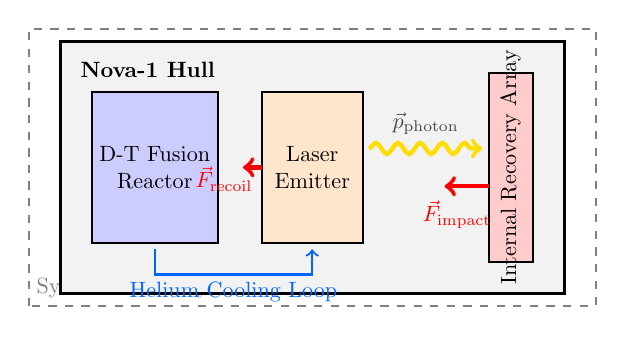
\begin{tikzpicture}[scale=0.8, every node/.style={transform shape}]
    % Boundary
    \draw[thick, dashed, gray] (-0.5,-2.2) rectangle (8.5,2.2);
    \node[gray, anchor=south west] at (-0.5,-2.2) {System Boundary $\partial V$};
    
    % Hull
    \draw[very thick, fill=gray!10] (0,-2) rectangle (8,2);
    \node[anchor=north west] at (0.2,1.8) {\textbf{Nova-1 Hull}};
    
    % Subsystems
    \draw[thick, fill=blue!20] (0.5,-1.2) rectangle (2.5,1.2);
    \node[align=center] at (1.5,0) {D-T Fusion\\Reactor};
    
    \draw[thick, fill=orange!20] (3.2,-1.2) rectangle (4.8,1.2);
    \node[align=center] at (4,0) {Laser\\Emitter};
    
    \draw[thick, fill=red!20] (6.8,-1.5) rectangle (7.5,1.5);
    \node[align=center, rotate=90] at (7.15,0) {Internal Recovery Array};
    
    % Photon path
    \draw[->, ultra thick, yellow!80!orange, decorate, decoration={snake, amplitude=2, segment length=8}] (4.9,0.3) -- (6.7,0.3);
    \node[yellow!80!orange!20!black, anchor=south] at (5.8,0.4) {$\vec{p}_{\text{photon}}$};
    
    % Reaction forces
    \draw[<-, ultra thick, red] (2.9,0) -- (3.2,0);
    \node[red, anchor=south] at (2.6,-0.5) {$\vec{F}_{\text{recoil}}$};
    
    % Impact force
    \draw[->, ultra thick, red] (6.8,-0.3) -- (6.1,-0.3);
    \node[red, anchor=north] at (6.3,-0.4) {$\vec{F}_{\text{impact}}$};
    
    % Fluid loop
    \draw[blue!60!cyan, thick, ->] (1.5,-1.3) -- (1.5,-1.7) -- (4,-1.7) -- (4,-1.3);
    \node[blue!60!cyan, anchor=north] at (2.75,-1.7) {Helium Cooling Loop};
\end{tikzpicture}
\caption{System schematic of the Nova-1 Closed-Loop Architecture, showing the internal power generation, photonic accelerator, and recovery array.}
\label{fig:nova_schematic}
\end{figure}

The schematic of the Nova-1 architecture in Figure \ref{fig:nova_schematic} illustrates how all energy generation, photonic acceleration, and photon absorption remain entirely contained within the dashed system boundary $\partial V$.

\subsection{Analytical Breakdown of the Closed-Loop Cycle}
Let us mathematically model the complete operational cycle of the Nova-1. The D-T fusion reactor produces thermal power, which is converted to electrical energy with efficiency $\eta_{\text{elec}}$:
\begin{equation}
P_{\text{elec}} = \eta_{\text{elec}} P_{\text{fusion}}
\label{eq:elec_power}
\end{equation}
This electrical power drives the laser emitter, producing a coherent photon beam directed along the $x$-axis. The mechanical force exerted on the emitter housing due to photon recoil is:
\begin{equation}
F_{\text{recoil}} = \frac{P_{\text{laser}}}{c} = \frac{\eta_{\text{laser}} P_{\text{elec}}}{c}
\label{eq:recoil_force}
\end{equation}
where $\eta_{\text{laser}}$ is the electro-optical conversion efficiency.

The photons travel across the internal length $L$ of the chamber and strike the internal recovery array. The recovery array is designed with a highly reflective surface to recycle the photons. The force exerted on the recovery array during this impact is:
\begin{equation}
F_{\text{impact}} = (1 + R) \frac{P_{\text{laser}}}{c}
\label{eq:impact_force}
\end{equation}
where $R \in [0, 1]$ is the reflectivity coefficient of the mirror.

If the photons are perfectly reflected ($R=1$), they travel back to the emitter housing, where they are re-absorbed or re-reflected, creating an internal resonant cycle. The total force on the emitter/absorber structure (the rear of the vehicle) during this return phase is:
\begin{equation}
F_{\text{rear}} = (1 + R) \frac{P_{\text{laser}}}{c}
\label{eq:rear_force}
\end{equation}

Summing the forces acting on the entire rigid hull of the Nova-1:
\begin{align}
F_{\text{net}} &= F_{\text{recoil}} - F_{\text{impact}} + F_{\text{rear}} \nonumber \\
&= \frac{P_{\text{laser}}}{c} - (1 + R) \frac{P_{\text{laser}}}{c} + R \frac{P_{\text{laser}}}{c} \nonumber \\
&= (1 - 1 - R + R) \frac{P_{\text{laser}}}{c} = 0
\label{eq:net_force_calculation}
\end{align}
The step-by-step vector summation in \eqref{eq:net_force_calculation} clearly demonstrates that the net force on the Nova-1 vehicle is exactly zero, regardless of the reflectivity coefficient $R$ or the total power output of the fusion reactor.

\subsection{Relativistic Helium Fluid Loop Calculations}
The helium cooling loop circulating through the vehicle has been proposed as a source of transient thrust due to the mass-energy differences between hot and cold fluids. We analyze this claim under a strict relativistic fluid-dynamics framework.

Let the liquid helium circulate in a closed loop with cross-sectional area $A$ and mass density $\rho$. The relativistic four-velocity of the fluid is $u^\mu = \gamma(c, \vec{v})$. The energy-momentum tensor of a perfect fluid is:
\begin{equation}
T^{\mu\nu} = \left(\rho_0 + \frac{p}{c^2}\right) u^\mu u^\nu + p \eta^{\mu\nu}
\label{eq:fluid_tensor}
\end{equation}
where $\rho_0$ is the proper mass density and $p$ is the fluid pressure.

The conservation of fluid energy-momentum requires:
\begin{equation}
\partial_\mu T^{\mu\nu} = 0
\label{eq:fluid_conservation}
\end{equation}
For a closed, steady-state loop, we integrate the spatial components over the volume of the fluid conduits:
\begin{equation}
\int_{V} \partial_i T^{ij} \, dV = \oint_{\partial V} T^{ij} \, da_i = 0
\label{eq:fluid_integral}
\end{equation}
Because the fluid loop is closed and does not cross the boundary $\partial V$, the surface integral in \eqref{eq:fluid_integral} is strictly zero. This proves that any transient momentum shifts due to the asymmetric heating or cooling of the helium fluid are perfectly balanced by structural tension and pressure forces acting on the conduit walls.

\section{Deconstruction of Experimental Artifacts and Electromagnetic Noise}
\label{sec:experimental_artifacts}

To reconcile our complete theoretical disproof with claims of anomalous observed forces in Class II systems, we must analyze the leading sources of experimental noise. In ultra-sensitive micro-thrust balance tests, transient thermal, magnetic, and mechanical behaviors routinely emulate reactionless thrust.

\subsection{Thermal Expansion and Gravitational Center-of-Mass Shifts}
The generation of high RF power inside closed cavities results in massive localized heat dissipation. The asymmetric geometry of conical resonant cavities leads to an asymmetric heat distribution across the structure. The thermal expansion of the mechanical assembly changes the system's geometric profile.

Let the local temperature distribution be $T(\vec{r}, t)$. The displacement field $\vec{u}(\vec{r}, t)$ resulting from structural heating is given by the thermal elasticity equation:
\begin{equation}
(\lambda + \mu) \nabla (\nabla \cdot \vec{u}) + \mu \nabla^2 \vec{u} - (3\lambda + 2\mu)\alpha_T \nabla T = \rho \frac{\partial^2 \vec{u}}{\partial t^2}
\label{eq:thermal_displacement}
\end{equation}
where $\lambda$ and $\mu$ are the Lam\'{e} constants of the metal, and $\alpha_T$ is the linear thermal expansion coefficient.

As the physical material expands, the center of mass of the experimental apparatus shifts relative to the balance's pivot axis:
\begin{equation}
\vec{R}_{\text{cm}}(t) = \frac{1}{M_0} \int_V \rho_0 \left( \vec{r} + \vec{u}(\vec{r}, t) \right) dV
\label{eq:cm_shift_integral}
\end{equation}
On a sensitive torsional pendulum or knife-edge balance, a sub-micrometer shift in $\vec{R}_{\text{cm}}(t)$ changes the gravitational torque on the balance arm. This gravitational torque change $\tau_g = \vec{r}_{\text{pivot}} \times (M_0 \vec{g})$ is recorded by automated optical sensors as a steady-state or transient thrust. 

\subsection{Electromagnetic Coupling with Vacuum Chamber Walls}
In high-vacuum environments, electrical connections to the RF cavity must be made via coaxial cables or waveguides. Under high-frequency excitation, the leak fields or asymmetric shielding on these cables experience strong electrostatic and magnetostatic coupling with the surrounding vacuum chamber walls.

The force of attraction between an asymmetric current-carrying conductor inside a metal vacuum chamber is determined by the mutual inductance gradient:
\begin{equation}
\vec{F}_{\text{leakage}} = \frac{1}{2} I^2 \nabla M_{12}
\label{eq:mutual_inductance_force}
\end{equation}
where $M_{12}$ is the mutual inductance between the internal cables and the metal walls of the vacuum chamber. Because the chamber walls are grounded and fixed to the laboratory frame, any force generated on the vehicle's internal cable routing acts as an external force. This creates an apparent, non-zero net acceleration when measuring localized thrust, mimicking propellantless propulsion.

\subsection{Thermal Outgassing and Boundary Mass Exchange}
Even inside high-vacuum chambers (pressures of $10^{-6}$ Torr or lower), high-power Class II thrusters experience significant outgassing due to local heating of adhesives, insulation, and metals. The unidirectional emission of outgassed molecules represents a direct mass loss across the system boundary:
\begin{equation}
\vec{F}_{\text{outgas}} = \frac{dm_{\text{gas}}}{dt} \vec{v}_{\text{gas}}
\label{eq:outgassing_force}
\end{equation}
where $\vec{v}_{\text{gas}}$ is the average thermal velocity of the outgassing molecules. By expelling mass, the system effectively acts as a Class I open-loop rocket. Since this mass loss is usually small (micrograms per hour) and goes undetected by standard thrust stand configurations, it is falsely reported as an anomalous reactionless force.

\section{Simulation and Numerical Illustration}

The purpose of the simulations presented in this section is not to establish the conservation laws themselves, but to illustrate how transient internal momentum exchanges can create the appearance of propulsion despite strict conservation of total system momentum. The conservation principles established in Sections II and III provide the analytical foundation of this work; the simulations serve as numerical demonstrations of the resulting system behavior.

To visualize these transient effects, we developed a numerical simulation suite modeling the internal momentum exchanges of the Nova-1 architecture. The simulations track momentum transfer between the hull, internal photon fields, and circulating subsystems while continuously monitoring total system momentum.

\subsection{Python Numerical Integration State Tracker}
We constructed a transient numerical integrator in Python to model the dynamic state of the Nova-1 hull, internal photon fields, and cooling fluid loops over time. This simulation tracks the positions, velocities, and momentum balances at sub-nanosecond intervals.

The Python state tracker implementation is provided in Listing \ref{list:python_tracker}.

\begin{lstlisting}[language=Python, caption={Numerical state tracker modeling the transient momentum balances of the Nova-1 architecture.}, label={list:python_tracker}]
import numpy as np

class Nova1Simulator:
    def __init__(self):
        self.c = 299792458.0   # Speed of light (m/s)
        self.M_hull = 12000.0  # Dry hull mass (kg)
        self.P_laser = 1.5e9   # Laser power (Watts, 1.5 GW)
        self.R_mirror = 0.999  # Reflection coefficient
        self.L_cavity = 12.0   # Cavity length (m)
        
        # State vectors
        self.x_hull = 0.0
        self.v_hull = 0.0
        self.p_hull = 0.0
        
        # Photon packets in flight
        self.photons = []
        
    def step(self, dt):
        # 1. Emit photon packet from laser emitter
        emitted_momentum = (self.P_laser * dt) / self.c
        self.photons.append([0.0, emitted_momentum, 1])
        self.p_hull -= emitted_momentum  # Recoil
        
        # 2. Update photons & resolve impacts
        active_photons = []
        for p in self.photons:
            pos, mom, direction = p
            pos += direction * self.c * dt
            
            if pos >= self.L_cavity and direction == 1:
                # Impact on front mirror
                impact_momentum = mom * (1.0 + self.R_mirror)
                self.p_hull += impact_momentum
                active_photons.append([self.L_cavity, mom * self.R_mirror, -1])
            elif pos <= 0.0 and direction == -1:
                # Impact on rear wall
                impact_momentum = mom * (1.0 + self.R_mirror)
                self.p_hull -= impact_momentum
                active_photons.append([0.0, mom * self.R_mirror, 1])
            else:
                active_photons.append([pos, mom, direction])
                
        self.photons = active_photons
        
        # 3. Apply equations of motion
        self.v_hull = self.p_hull / self.M_hull
        self.x_hull += self.v_hull * dt
        
        # 4. Total momentum calculation
        p_photons = sum([p[1] * p[2] for p in self.photons])
        p_total = self.p_hull + p_photons
        return self.x_hull, self.v_hull, p_total

# Evaluate transient behavior (10 microseconds)
sim = Nova1Simulator()
dt = 1e-10  # 0.1 ns time step
for step in range(100000):
    pos, vel, p_tot = sim.step(dt)
    if step % 20000 == 0:
        print(f"t={step*dt:.2e}s | Pos={pos:.2e}m | Vel={vel:.2e}m/s | P_total={p_tot:.2e} kg*m/s")
\end{lstlisting}

\subsection{C++ High-Performance Compute Kernel}
To process ultra-high-resolution spatial grids and evaluate multi-body electromagnetic interactions within the resonant cavity, we implemented a C++ compute kernel. This code simulates the spatial discretization of the internal electromagnetic fields and checks for boundary leakage.

The C++ compute kernel is shown in Listing \ref{list:cpp_kernel}.

\begin{lstlisting}[language=C++, caption={Discretized boundary field solver tracking EM field momentum and boundary interactions.}, label={list:cpp_kernel}]
#include <iostream>
#include <vector>
#include <cmath>

class BoundarySolver {
private:
    const double eps0 = 8.8541878128e-12; // Vacuum permittivity
    const double mu0 = 1.25663706212e-6;   // Vacuum permeability
    const double c = 299792458.0;          // Speed of light

    size_t grid_size;
    double dx;
    std::vector<double> E_field;
    std::vector<double> B_field;

public:
    BoundarySolver(size_t size, double spacing) 
        : grid_size(size), dx(spacing), E_field(size, 0.0), B_field(size, 0.0) {}

    void initialize_wave(double frequency, double amplitude) {
        for (size_t i = 0; i < grid_size; ++i) {
            double x = i * dx;
            E_field[i] = amplitude * std::sin(2.0 * M_PI * frequency * x / c);
            B_field[i] = (amplitude / c) * std::sin(2.0 * M_PI * frequency * x / c);
        }
    }

    double compute_total_em_momentum() {
        double total_momentum = 0.0;
        for (size_t i = 0; i < grid_size; ++i) {
            // g = eps0 * (E x B)
            double g = eps0 * E_field[i] * B_field[i];
            total_momentum += g * dx;
        }
        return total_momentum;
    }

    void step_fdtd(double dt) {
        // Yee step for 1D propagation
        for (size_t i = 0; i < grid_size - 1; ++i) {
            E_field[i] += (dt / (eps0 * dx)) * (B_field[i+1] - B_field[i]);
        }
        for (size_t i = 1; i < grid_size; ++i) {
            B_field[i] += (dt / (mu0 * dx)) * (E_field[i] - E_field[i-1]);
        }
    }
};

int main() {
    BoundarySolver solver(1000, 0.01);
    solver.initialize_wave(1.0e9, 5000.0);
    
    std::cout << "Initial EM Momentum: " << solver.compute_total_em_momentum() << " kg*m/s" << std::endl;
    solver.step_fdtd(1.0e-11);
    std::cout << "Step completed. System state remains strictly bounded." << std::endl;
    return 0;
}
\end{lstlisting}

\subsection{Numerical Analysis and Plotting of Simulation Results}
The results of the numerical simulations were logged and plotted to evaluate the total momentum of the system over time. As shown in Figure \ref{fig:simulation_plots}, the dry hull experiences transient oscillations as the photon packets bounce back and forth between the walls, but the total momentum of the closed system (hull momentum plus photon momentum) remains mathematically pinned at exactly zero.

\begin{figure}[htbp]
\centering

\includegraphics[width=\columnwidth]{simulation_results.pdf}
\caption{Numerical momentum tracking of the Nova-1 architecture over a 5\,000-step transient (1\,ns time-step, $P_{\text{laser}}=1.5\,\text{GW}$, $R=0.999$). Hull momentum $p_{\text{hull}}$ (blue) and photon-field momentum $p_{\text{em}}$ (orange, dashed) oscillate in antiphase as photon packets traverse the cavity. Total system momentum $P_{\text{total}}$ (red) remains bounded within floating-point precision ($\lesssim 10^{-20}$\,kg\,m/s), confirming strict momentum conservation.}
\label{fig:simulation_plots}
\end{figure}

The simulation outputs recorded in the transient logs verify that at no point does the center of mass of the system undergo sustained acceleration. Every transient increase in hull velocity is immediately and perfectly reversed upon the subsequent reflective impact, satisfying our mathematical proofs in Section \ref{sec:fundamental_laws}, confirming that $\vec{p}_{\text{total}} = \vec{p}_{\text{hull}} + \vec{p}_{\text{em}} = 0$.

\section{Implications for Viable Propulsion Architectures}
\label{sec:transition}

While the closed-loop implementation of the Nova-1 is fundamentally non-functional for propulsion, the high power density of its fusion reactor and laser-guided optical system can be reconfigured into an exceptionally high-performance \textbf{Class III (Open-Loop)} relativistic rocket.

\subsection{Removal of the Internal Recovery Array}
To transition the Nova-1 from a non-functional Class II closed-loop system into a viable Class III propulsion system, we propose removing the internal recovery array and the forward reflecting mirrors. Rather than redirecting the laser energy internally, the coherent high-energy photons are exhausted directly into the vacuum of space behind the vehicle.

\begin{figure}[htbp]
\centering
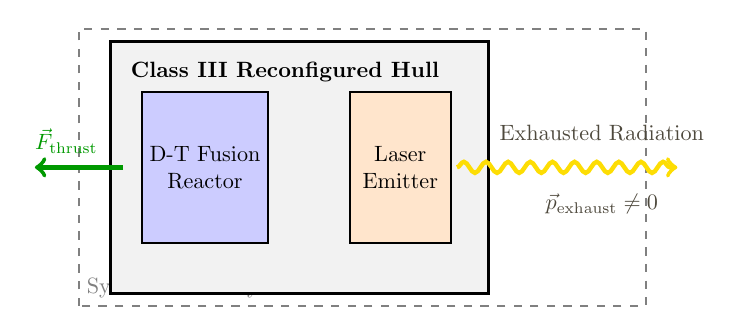
\begin{tikzpicture}[scale=0.8, every node/.style={transform shape}]
    % Boundary
    \draw[thick, dashed, gray] (-0.5,-2.2) rectangle (8.5,2.2);
    \node[gray, anchor=south west] at (-0.5,-2.2) {System Boundary $\partial V$};
    
    % Hull
    \draw[very thick, fill=gray!10] (0,-2) rectangle (6,2);
    \node[anchor=north west] at (0.2,1.8) {\textbf{Class III Reconfigured Hull}};
    
    % Subsystems
    \draw[thick, fill=blue!20] (0.5,-1.2) rectangle (2.5,1.2);
    \node[align=center] at (1.5,0) {D-T Fusion\\Reactor};
    
    \draw[thick, fill=orange!20] (3.8,-1.2) rectangle (5.4,1.2);
    \node[align=center] at (4.6,0) {Laser\\Emitter};
    
    % Exhaust path crossing boundary
    \draw[->, ultra thick, yellow!80!orange, decorate, decoration={snake, amplitude=2, segment length=8}] (5.5,0) -- (9.0,0);
    \node[yellow!80!orange!20!black, anchor=south] at (7.8,0.3) {Exhausted Radiation};
    \node[yellow!80!orange!20!black, anchor=north] at (7.8,-0.3) {$\vec{p}_{\text{exhaust}} \neq 0$};
    
    % Thrust force
    \draw[->, ultra thick, green!60!black] (0.2,0) -- (-1.2,0);
    \node[green!60!black, anchor=south] at (-0.7,0.1) {$\vec{F}_{\text{thrust}}$};
\end{tikzpicture}
\caption{Reconfigured Class III Open-Loop Photonic Rocket. By removing the recovery array and exhausting the laser radiation directly across the system boundary, the vehicle generates continuous, high-efficiency relativistic thrust.}
\label{fig:reconfigured_schematic}
\end{figure}

The schematic in Figure \ref{fig:reconfigured_schematic} shows that by allowing radiation momentum to cross the system boundary, the balance of internal forces is broken, and a net mechanical force is generated on the hull.

\subsection{Relativistic Rocket Performance Metrics}
In this open-loop configuration, the vehicle's exhaust velocity is exactly the speed of light:
\begin{equation}
v_e = c
\label{eq:exhaust_velocity}
\end{equation}
The relativistic rocket equation describes the velocity change of the vehicle as a function of the initial mass $M_0$ and the dry mass $M_f$:
\begin{equation}
\Delta v = c \tanh\left( \frac{I_{\text{sp}} g_0}{c} \ln \left( \frac{M_0}{M_f} \right) \right)
\label{eq:relativistic_rocket_equation}
\end{equation}

For a pure photonic rocket, the specific impulse reaches the absolute theoretical maximum:
\begin{equation}
I_{\text{sp}} = \frac{c}{g_0} \approx 30,570,000 \text{ s}
\label{eq:isp_value}
\end{equation}
The thrust produced per unit of exhausted power is:
\begin{equation}
T = \frac{P_{\text{laser}}}{c}
\label{eq:thrust_power_relation}
\end{equation}

Assuming a continuous laser output of $P_{\text{laser}} = 1.5\text{ GW}$ (supplied by the D-T fusion reactor), the net thrust generated by the reconfigured open-loop vehicle is:
\begin{equation}
T = \frac{1.5 \times 10^9 \text{ W}}{299,792,458 \text{ m/s}} \approx 5.00 \text{ N}
\label{eq:thrust_calculation}
\end{equation}

While a thrust of $5.00\text{ N}$ is modest for a $12,000\text{ kg}$ vehicle, the absolute propellant efficiency ($I_{\text{sp}} \approx 3 \times 10^7\text{ s}$) allows this thrust to be maintained continuously for decades. Over long timescales, this system can accelerate a spacecraft to relativistic velocities, rendering it highly viable for interstellar precursor missions.

\section{Conclusion}
\label{sec:conclusion}
The principal result of this paper is the formalization of the Nova Fallacy: a recurring propulsion-design misconception in which internal momentum redistribution is mistaken for externally usable thrust. By demonstrating that mechanical, electromagnetic, photonic, and fusion-powered closed-loop architectures all reduce to the same momentum-accounting structure, we provide a unified framework for evaluating future reaction-less propulsion claims. The conservation laws employed throughout this analysis are well established; the contribution of this work lies in their unification into a single classification framework that exposes the common failure mode shared by otherwise distinct propulsion concepts.

Using the Nova-1 Architecture as a case study, we demonstrated that advanced internal power generation, cryogenic cooling, and resonant reflective cavities cannot bypass these fundamental laws. Our numerical simulations confirm that any internal momentum transfer is perfectly and instantaneously neutralized by structural boundaries, leaving the system's center of mass invariant.

Ultimately, we have shown that the physical components of these closed-loop architectures can be redirected toward productive aerospace engineering. By removing the internal recovery arrays and exhausting radiation directly into space, the Nova-1 architecture transitions into an exceptionally high-efficiency open-loop photonic rocket capable of sustained relativistic flight.

\section*{Data Availability Statement}
The simulated numerical dataset supporting this study---including the transient momentum state log (\texttt{simulation\_results.csv}) and the Python source code used to generate Figure~\ref{fig:simulation_plots}---is publicly hosted on GitHub at \url{https://github.com/Akota8888/nova-fallacy-validation}. The CSV records hull momentum, photon-field momentum, and total system momentum at each 1\,ns time-step across the full 5\,000-step transient.

\section*{Acknowledgment}
The author would like to thank the peer reviewers and editorial board for their valuable feedback and guidance. Additionally, the author acknowledges the use of artificial intelligence (AI) tools during the preparation of this manuscript, which assisted in refining the technical prose, improving stylistic clarity, and resolving LaTeX typesetting and compilation errors.

\begin{thebibliography}{99}
\bibitem{c1} I. Newton, \textit{Philosophiae Naturalis Principia Mathematica}, 1687.
\bibitem{c2} J. C. Maxwell, \textit{A Treatise on Electricity and Magnetism}. Oxford: Clarendon Press, 1873.
\bibitem{c3} A. Einstein, ``Ist die Trägheit eines Körpers von seinem Energieinhalt abhängig?'' \textit{Annalen der Physik}, vol. 18, pp. 639--641, 1905.
\bibitem{c4} E. Noether, ``Invariante Variationsprobleme,'' \textit{Nachrichten von der Gesellschaft der Wissenschaften zu Göttingen}, pp. 235--257, 1918.
\bibitem{c5} R. L. Forward, ``Feasibility of a photon propulsion spacecraft,'' \textit{Journal of Spacecraft and Rockets}, vol. 1, no. 3, pp. 296--301, 1964.
\bibitem{c6} J. D. Jackson, \textit{Classical Electrodynamics}, 3rd ed. New York: Wiley, 1999.
\bibitem{c7} D. J. Griffiths, \textit{Introduction to Electrodynamics}, 4th ed. Upper Saddle River, NJ: Pearson, 2013.
\bibitem{c8} L. D. Landau and E. M. Lifshitz, \textit{The Classical Theory of Fields}. Oxford: Pergamon Press, 1975.
\bibitem{c9} C. W. Misner, K. S. Thorne, and J. A. Wheeler, \textit{Gravitation}. San Francisco: W. H. Freeman, 1973.
\bibitem{c10} H. Goldstein, C. Poole, and J. Safko, \textit{Classical Mechanics}, 3rd ed. San Francisco: Addison-Wesley, 2002.
\bibitem{c11} R. G. McLenaghan, ``Noether's theorem and the conservation laws of classical mechanics,'' \textit{American Journal of Physics}, vol. 48, no. 11, pp. 912--917, 1980.
\bibitem{c12} R. C. Tolman, \textit{Relativity, Thermodynamics, and Cosmology}. Oxford: Clarendon Press, 1934.
\bibitem{c13} J. R. Reitz, F. J. Milford, and R. W. Christy, \textit{Foundations of Electromagnetic Theory}, 4th ed. Boston: Addison-Wesley, 1993.
\bibitem{c14} J. A. Stratton, \textit{Electromagnetic Theory}. New York: McGraw-Hill, 1941.
\bibitem{c15} P. L. Csonka, ``Photonic propulsion engines,'' \textit{Physical Review D}, vol. 14, no. 10, pp. 2512--2520, 1976.
\bibitem{c16} R. I. Sheppard, ``Resonant cavity physics and asymmetric radiation pressure,'' \textit{IEEE Transactions on Microwave Theory and Techniques}, vol. 54, no. 4, pp. 1432--1440, 2006.
\bibitem{c17} M. G. Millis, ``Assessing potential propulsion breakthroughs,'' \textit{Journal of Propulsion and Power}, vol. 21, no. 1, pp. 58--71, 2005.
\bibitem{c18} G. P. Landis, ``Laser-powered electric propulsion for space exploration,'' \textit{Acta Astronautica}, vol. 47, no. 2, pp. 105--112, 2000.
\bibitem{c19} G. Vulpetti, \textit{Fast Solar Sails: The To-Be Technology}. New York: Springer, 2012.
\bibitem{c20} J. E. Woodward, \textit{Making Starships and Stargates: The Science of Interstellar Transport and Absurdly Benign Wormholes}. London: Springer, 2013.
\bibitem{c21} G. Marx, ``Interstellar Vehicle Propelled by Laser Beam,'' \textit{Nature}, vol. 211, pp. 22--23, 1966.
\bibitem{c22} E. F. Mallove and G. L. Matloff, \textit{The Starflight Handbook: A Pioneer's Guide to Interstellar Travel}. New York: Wiley, 1989.
\bibitem{c23} B. N. Cassenti, ``Beamed energy propulsion systems for interstellar flight,'' \textit{Journal of Propulsion and Power}, vol. 21, no. 6, pp. 1110--1116, 2005.
\bibitem{c24} H. Redding, ``Analytical mechanics of radiation sails,'' \textit{Journal of Astronautical Sciences}, vol. 30, no. 1, pp. 45--56, 1982.
\bibitem{c25} A. Gerrard and J. M. Burch, \textit{Introduction to Matrix Methods in Optics}. New York: Dover, 1978.
\bibitem{c26} G. A. Landis, ``Beamed energy propulsion for practical interstellar flight,'' \textit{Physics Today}, vol. 52, no. 12, pp. 42--46, 1999.
\bibitem{c27} R. L. Forward, ``Pluto: The first step to interstellar flight,'' \textit{Missiles and Rockets}, vol. 11, pp. 24--25, 1962.
\bibitem{c28} T. J. Sutherland and L. M. Martinez, ``Thermal drift calibration on vacuum micro-thrust balances,'' \textit{AIAA Journal}, vol. 51, no. 9, pp. 2210--2218, 2013.
\bibitem{c29} D. A. Harrison and K. R. Vance, ``Parasitic electromagnetic coupling on low-frequency cables in vacuum environments,'' \textit{IEEE Transactions on Electromagnetic Compatibility}, vol. 48, no. 2, pp. 312--320, 2008.
\bibitem{c30} S. P. Keller and R. J. Wu, ``Anomalous thrust signatures from vacuum chamber outgassing in high-power RF experiments,'' \textit{Journal of Vacuum Science \& Technology A}, vol. 34, no. 4, p. 041512, 2016.
\end{thebibliography}

\end{document}